\section{Method}


% Tigo
\subsection{Movement of the explorer bot}
The explorer bot is designed to navigate autonomously in an indoor environment, utilizing omniwheels for movement.
To evaluate the performance of omniwheels in robotic movement, a test platform was designed and constructed. The platform consists of the following components:

\begin{itemize}
    \item \textbf{Omniwheels}: Three omniwheels arranged in a triangular configuration to enable omnidirectional movement.
    \item \textbf{Motors \& Drivers}: Each wheel is powered by a DC motor, controlled via two \textbf{L298N (HW-95) motor drivers}, ensuring precise speed and direction control.
    \item \textbf{Microcontrollers \& Communication}:
    \begin{itemize}
        \item An \textbf{ESP32 UWB} serves as the \textbf{master controller}, responsible for high-level motion commands and data collection.
        \item A secondary \textbf{ESP32} acts as a \textbf{slave controller}, handling motor control and executing movement instructions in real time.
    \end{itemize}
    \item \textbf{Power Supply}: Two different battery packs. One is for the master controller and the other is for the slave controller and motors.
\end{itemize}

\subsection{Hardware Design}

The hardware design consists of the integration of omniwheels, motors, motor drivers, ESP32 microcontrollers, and a dual power supply system. The master ESP32 UWB handles high-level motion commands and data processing, while the slave ESP32 executes real-time motor control. The wiring connections between the ESP32 boards, motor drivers, and power supply are illustrated in Figure \ref{fig:motoropstelling}.

\begin{figure}[h]
    \centering
    \caption{Motor Driver and ESP32 Wiring Diagram}
    \label{fig:motoropstelling}
    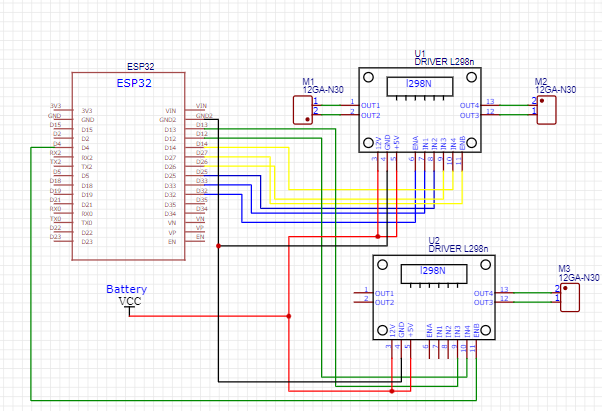
\includegraphics[width=0.5\textwidth]{motoropstelling.png}
\end{figure}


% Thomas

\subsection{The display}
The explorer bot uses a lcd display to show basic information to the 
user. The chosen display makes use of the i2c protocol to communicate 
with the microcontroller (I2c allows multiple devices to be connected to
the same two wires which simplifies connections). 
The display was connected to an ESP32 microcontroller to test it in the 
same way it will be used in the final product. These connections are found 
in the electric schematic in the appendix. For testing purposes a test 
program was 
created which shows a text on the display with an number behind it which 
increments once every 500 miliseconds.
To test the display the test code is uploaded to the ESP32 and the display was
monitored until the number on the display reached to 10 to see if the correct text is displayed.  % \ref{app:schematic}
Following the above procedure the display was tested and found to be working. 

\subsection{The gyroscope sensor}
The explorer bot will need to know its orientation to correctly interpret 
sensor data (--see other subsection--). For this reason an i2c gyroscope 
sensor was chosen. The gyroscope was connected to the ESP32 microcontroller 
according to the electric schematic in the appendix (TODO) and testcode was 
written which prints the sensor data in the terminal. This test code was 
uploaded to the ESP32 and the sensor was rotated on the x, y and z axis to 
see if the sensor data changes accordingly. The sensor was found to 
be working correctly.
Later the gyroscope sensor was replaced by a magnetometer sensor

% Toine
The robot uses ultrasonic sensors to measure the distance to the nearest object. Using these values, we can draw lines on the map to define the room and obstacles.
During testing, we encountered an issue we had not initially accounted for: when the robot rotates, the sensors rotate with it. 
This means we need to track the robot's rotation relative to its starting position. Using this rotation, we can adjust the sensor readings accordingly. 
For example, if the robot has turned 30 degrees, the measured distances must be transformed to match the new orientation.
To perform these calculations, we use the Pythagorean theorem along with trigonometric functions to accurately determine the position of obstacles. 
The Pythagorean theorem is particularly useful for recalculating distances when translating between coordinate systems after rotation.
We started testing by first verifying the accuracy of the ultrasonic sensors. This was done by placing an object at a predefined distance from the 
sensor and comparing the measured values with the expected results. We printed the raw sensor data to confirm the measurements were correct. Once we 
validated the sensor readings, we focused on determining the robot's rotation angle.
Initially, we considered using a gyroscope, as it seemed like a suitable solution. However, after extensive testing, we discovered that the gyroscope 
primarily measures angular velocity around the X and Y axes rather than absolute rotation around the Z-axis. Despite this limitation, we used the 
gyroscope to test real-time recalculations of sensor data. By manually rotating the sensor and observing the calculated angle, raw sensor data, and 
recalculated distances, we verified the correctness of our approach. Once this was confirmed, we replaced the gyroscope with a magnetometer, which 
provided direct measurements of the robot's heading.





% Overzicht totale systeem: architectuurontwerp en data flow-ontwerp (groepswerk). Gebruik vooral ook plaatjes en schema's. Voor plaatjes worden in \LaTeX{} ``drijvende'' figuren (\textsl{floats}) gebruikt. 
% Deze drijven naar de bovenkant van de pagina, of naar de volgende pagina, zodat de tekst niet onderbroken wordt. Een voorbeeld is figuur~\ref{doos}.
% \begin{figure}[b] % drijvend figuur
% \caption{Dit is het onderschrift bij een drijvend figuur.} % onderschrift, wordt automatisch genummerd
% \label{doos} % label om naar figuur te verwijzen
% \end{figure}

% \end{flushright}